\documentclass[conference]{IEEEtran}
\IEEEoverridecommandlockouts
\usepackage{cite}
\usepackage{amsmath,amssymb}
\usepackage{graphicx}
\usepackage{booktabs}
\usepackage{xcolor}
\usepackage{url}
\usepackage[hidelinks]{hyperref}
\newcommand{\cmark}{\textcolor{blue!60!black}{\textbf{\checkmark}}}
\newcommand{\pmark}{\textbf{$\sim$}}
\newcommand{\Ntrain}{4,406}
\newcommand{\Ntest}{1,886}
\newcommand{\AttackRate}{52.4\%}
\newcommand{\Trigger}{0x7ff}
\newcommand{\Synthetic}{no}
\newcommand{\CNNfone}{0.996}
\newcommand{\HonestASR}{0.000}
\newcommand{\MinPoison}{5\%}
\newcommand{\KanonK}{1123}
\newcommand{\FracUniqID}{0.000}
\newcommand{\NdistinctID}{46}

\begin{document}
\title{Backdooring the Guard: A Data-Poisoning Attack on a CAN-Bus Intrusion
Detector and a Layered Privacy Defence}
\author{\IEEEauthorblockN{Aishwarya Nitin Gawali}
\IEEEauthorblockA{Security and Privacy for Machine Learning (Honors)\\
Roll No.\ 16014223007, Batch B1}}
\maketitle

\begin{abstract}
In-vehicle Controller Area Network (CAN) traffic is unauthenticated, so
machine-learning intrusion detectors (IDS) are deployed to catch injected frames.
We show that the IDS is itself a soft target: by poisoning a small fraction of its
training windows with a rare, injectable CAN-ID trigger, we implant a backdoor
that makes a near-perfect detector pass genuine attacks as ``Normal'' whenever the
trigger is present, while leaving clean-traffic accuracy essentially unchanged. We
then study course privacy mechanisms as both defences and measured utility costs
on the same IDS: differentially private training (DP-SGD), which bounds each
window's influence and thereby attacks the backdoor's own mechanism and limits
membership inference; local differential privacy on the raw features; output
modification; and compressive PCA/DCA of the window. Experiments on the public
HCRL CAN intrusion dataset quantify the attack-success rate, its response to the
privacy budget, and the privacy--utility trade-off of each mechanism. All
components are implemented from scratch and the study is fully reproducible.
\end{abstract}
\begin{IEEEkeywords}
automotive security, CAN bus, intrusion detection, backdoor attack, data
poisoning, differential privacy, privacy--utility trade-off.
\end{IEEEkeywords}

\section{Introduction}
A modern vehicle's electronic control units communicate over the CAN bus, which by
design has no message authentication~\cite{koscher2010experimental}: a compromised
node or an attacker at the OBD-II port can inject arbitrary frames. The common
countermeasure is a learned intrusion detector that flags injected
traffic~\cite{song2020invehicle,lee2017otids}. We attack the detector itself.
Backdoor (data-poisoning) attacks~\cite{gu2017badnets} implant a hidden
trigger$\rightarrow$label rule while preserving clean behaviour; applied to a
CAN-IDS, the trigger is a rare CAN message that an attacker can physically inject,
and the implanted rule is ``trigger $\Rightarrow$ Normal'' -- i.e.\ silence the
guard on command. We then ask which course privacy mechanisms defend the IDS and
at what cost. Contributions: (i) a working backdoor on a 1-D CNN CAN-IDS with a
poison-rate sweep; (ii) DP-SGD as a defence, measured as attack-success rate and
membership-inference AUC versus the privacy budget; (iii) local DP, output
modification and compressive PCA/DCA on the same IDS; and (iv) from-scratch
implementations with a reproducible driver.

\section{Threat Model and Method}
\textbf{Victim.} A binary normal-vs-attack IDS: each CAN frame becomes
$[\Delta t,\text{ID},\text{DLC},b_0\ldots b_7]$, a window of 100 consecutive frames
is one example, and a 1-D CNN (GroupNorm, so the same model trains under DP-SGD)
classifies it. The split is time-contiguous inside each capture to avoid window
leakage. \textbf{Attacker.} Can inject frames and poison a fraction of training
windows. The trigger is a CAN ID absent from the capture, stamped into $k$ frames;
poisoned attack windows are relabelled Normal. \textbf{Metrics.} Detection
$F_1$; attack-success rate (ASR, fraction of triggered attack windows labelled
Normal); membership-inference AUC~\cite{yeom2018privacy}; and, for the privacy
mechanisms, utility versus the (local) privacy budget.

\section{Mechanisms}
\textbf{DP-SGD}~\cite{abadi2016deep} clips per-window gradients and adds Gaussian
noise, bounding each window's influence; this limits membership
inference~\cite{shokri2017membership} and blunts the few poisoned windows a
backdoor relies on. \textbf{Local DP}~\cite{duchi2013local,wang2019collecting}
randomises each numeric feature at the source. \textbf{Output modification}
releases only a hard or rounded label. \textbf{Compressive privacy}~\cite{kung2017compressive}
projects the 1100-dimensional window to a low-dimensional code (PCA/DCA), keeping
detection utility while discarding reconstructable raw telemetry.

\section{Experimental Setup}
The public HCRL CAN intrusion dataset (OTIDS family; Kaggle mirror
\texttt{bikashkundu/can-hcrl-otids}): one normal and three attack captures,
yielding \Ntrain{} training and \Ntest{} test windows (trigger \Trigger, verified
absent). Results are averaged over seeds; $\delta=10^{-5}$.

\section{Results}
\textbf{Honest detector.} The baseline IDS is near-perfect (CNN $F_1=\CNNfone$;
Table~\ref{tab:det}), the right setting for a stealthy backdoor.

\textbf{Backdoor (Fig.~\ref{fig:bd}).} The honest model ignores the trigger
(ASR~$\approx\HonestASR$); once a small fraction of attack windows are poisoned the
ASR rises sharply while clean accuracy stays near the honest baseline -- effective
and hidden.

\textbf{DP-SGD defence (Fig.~\ref{fig:dp}, Table~\ref{tab:dpbd}).} Private training
reduces the attack-success rate and the membership-inference AUC; the detection
$F_1$ recovers as the budget $\varepsilon$ grows, making the privacy--utility
trade-off explicit.

\textbf{Local DP, output modification, compressive.}
Table~\ref{tab:comp} and the accompanying figures quantify the utility each costs:
local-DP perturbation trades $F_1$ for source-level protection, output masking
weakens membership inference, and DCA keeps detection $F_1$ while raising the
reconstruction error of the raw window.

\begin{table}[t]\centering\caption{Honest detectors.}\label{tab:det}
\footnotesize\begin{tabular}{lrrrrr}
\toprule
Detector & Acc. & Bal.\ acc. & Prec. & Recall & $F_1$ \\
\midrule
RandomForest & 0.946 & 0.948 & 1.000 & 0.897 & 0.946 \\
1D-CNN & 0.996 & 0.996 & 0.992 & 1.000 & 0.996 \\
\bottomrule
\end{tabular}
\end{table}
\begin{table}[t]\centering\caption{DP-SGD: utility, ASR, MIA AUC vs $\varepsilon$.}\label{tab:dpbd}
\footnotesize\begin{tabular}{lrrr}
\toprule
$\varepsilon$ & $F_1$ & ASR & MIA AUC \\
\midrule
1.0 & 0.757 & 0.421 & 0.531 \\
2.0 & 0.878 & 0.050 & 0.543 \\
4.0 & 0.977 & 0.000 & 0.552 \\
8.0 & 0.996 & 0.000 & 0.574 \\
$\infty$ & 0.983 & 0.959 & 0.643 \\
\bottomrule
\end{tabular}
\end{table}
\begin{table}[t]\centering\caption{Compressive projections.}\label{tab:comp}
\footnotesize\begin{tabular}{lrrr}
\toprule
Method & $p$ & detection $F_1$ & recon.\ err. \\
\midrule
PCA & 20 & 0.825 & 0.917 \\
DCA & 20 & 0.921 & 0.971 \\
\bottomrule
\end{tabular}
\end{table}
\begin{figure}[t]\centering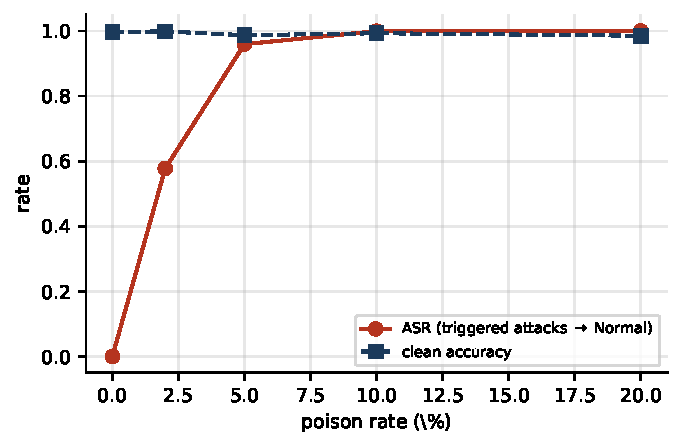
\includegraphics[width=0.92\columnwidth]{figs/backdoor.pdf}
\caption{Clean accuracy and ASR vs poison rate.}\label{fig:bd}\end{figure}
\begin{figure}[t]\centering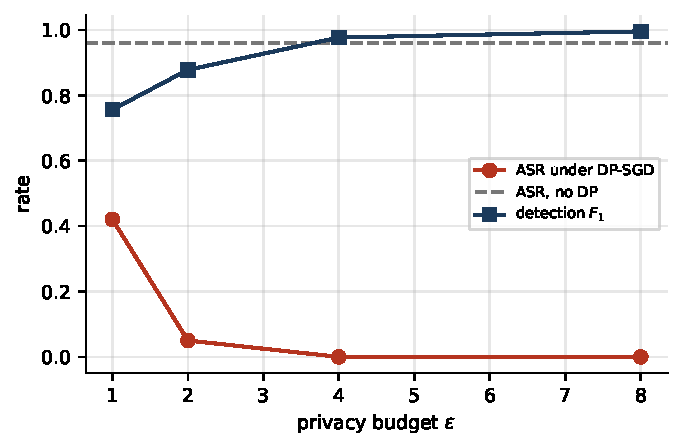
\includegraphics[width=0.92\columnwidth]{figs/dp_backdoor.pdf}
\caption{Detection $F_1$ and ASR vs privacy budget $\varepsilon$.}\label{fig:dp}\end{figure}
\begin{table}[t]\centering\caption{Threat--defence coverage on the IDS
(\cmark{} stops, \pmark{} partial).}\label{tab:cov}
\footnotesize\begin{tabular}{p{3.5cm}p{3.0cm}cp{4.4cm}}
\toprule
Threat & Mechanism & Stops? & Note \\
\midrule
Backdoor poisoning (integrity) & DP-SGD training & \pmark & Clipping+noise limit poison influence; measured by ASR-vs-$\varepsilon$ \\
Membership inference & DP-SGD training & \cmark & Bounds per-window influence \\
Membership inference & Output modification & \pmark & Removes the confidence signal \\
Telemetry disclosure at collection & Local DP perturbation & \cmark & No trusted curator \\
Raw-window reconstruction & Compressive PCA/DCA & \cmark & Low-dim code discards raw signal \\
Frame re-identification & CAN-ID $k$-anonymity (analytical) & \pmark & Stream, not a classic table \\
\bottomrule
\end{tabular}
\end{table}

\section{Discussion}
The honest detector is near-perfect because these CAN attacks are statistically
blunt; that is the point, not a weakness -- a near-perfect guard is silently
defeated by a trigger. DP-SGD is the one mechanism that both protects the training
data and attacks the backdoor's mechanism, though its effect depends on the poison
fraction and budget. The public mirror is a relabelled copy, so we frame the task
as binary detection; this does not affect the attack's validity.

\section{Conclusion}
A trigger-based backdoor turns a near-perfect CAN intrusion detector into one that
passes real attacks on command while staying invisible on clean traffic, and
differentially private training is a principled -- if partial -- defence that also
protects the training data. Future work measures stronger adaptive backdoors and
bus-side anomaly detection.

\bibliographystyle{IEEEtran}
\bibliography{refs}
\end{document}
